\documentclass[12pt, a4paper]{article}

% ─── Packages ────────────────────────────────────────────────────────────────
\usepackage[T1]{fontenc}
\usepackage[utf8]{inputenc}
\usepackage[margin=2.5cm, top=3cm, bottom=3cm]{geometry}
\usepackage{xcolor}
\usepackage{titlesec}
\usepackage{titling}
\usepackage{fancyhdr}
\usepackage{booktabs}
\usepackage{array}
\usepackage{tabularx}
\usepackage{colortbl}
\usepackage{amsmath}
\usepackage{amssymb}
\usepackage{graphicx}
\usepackage{hyperref}
\usepackage{parskip}
\usepackage{enumitem}
\usepackage{tcolorbox}
\usepackage{mdframed}
\usepackage{listings}
\usepackage{caption}
\usepackage{subcaption}
\usepackage{float}
\usepackage{setspace}
\usepackage{tikz}
\usetikzlibrary{shapes.geometric, arrows.meta, positioning, fit, backgrounds, calc, shadows}

% ─── Color Palette ────────────────────────────────────────────────────────────
\definecolor{primary}{RGB}{31, 73, 125}
\definecolor{secondary}{RGB}{0, 112, 192}
\definecolor{accent}{RGB}{192, 0, 0}
\definecolor{lightblue}{RGB}{219, 233, 246}
\definecolor{lightgray}{RGB}{245, 245, 245}
\definecolor{darkgray}{RGB}{64, 64, 64}
\definecolor{medgray}{RGB}{130, 130, 130}
\definecolor{tablehead}{RGB}{31, 73, 125}
\definecolor{rulecolor}{RGB}{0, 112, 192}
\definecolor{codebg}{RGB}{248, 249, 250}
\definecolor{noteboxbg}{RGB}{255, 248, 230}
\definecolor{noteborder}{RGB}{200, 150, 0}
\definecolor{warningbg}{RGB}{253, 236, 234}
\definecolor{warningborder}{RGB}{192, 0, 0}
\definecolor{webgreen}{RGB}{0, 128, 80}
\definecolor{webbg}{RGB}{230, 247, 238}
% TikZ node colors
\definecolor{tikzblue}{RGB}{31, 73, 125}
\definecolor{tikzlightblue}{RGB}{180, 210, 240}
\definecolor{tikzgreen}{RGB}{0, 128, 80}
\definecolor{tikzlightgreen}{RGB}{200, 235, 215}
\definecolor{tikzred}{RGB}{192, 0, 0}
\definecolor{tikzlightred}{RGB}{250, 215, 215}
\definecolor{tikzgold}{RGB}{180, 130, 0}
\definecolor{tikzlightgold}{RGB}{255, 245, 200}
\definecolor{tikzgray}{RGB}{90, 90, 90}
\definecolor{tikzlightgray}{RGB}{235, 235, 235}

% ─── Hyperref setup ───────────────────────────────────────────────────────────
\hypersetup{
  colorlinks=true,
  linkcolor=secondary,
  citecolor=primary,
  urlcolor=secondary,
  pdftitle={Multilingual Legal Chatbot --- RAG Architecture},
  pdfauthor={Bettayeb Mohamed Aimen, Amina, Yanis, Loubna},
}

% ─── Section Styling ──────────────────────────────────────────────────────────
\titleformat{\section}
  {\color{primary}\large\bfseries}
  {\color{secondary}\thesection.}{0.6em}{}
  [\vspace{-0.3em}\color{rulecolor}\rule{\linewidth}{0.8pt}\vspace{0.3em}]

\titleformat{\subsection}
  {\color{primary}\normalsize\bfseries}
  {\color{secondary}\thesubsection}{0.6em}{}

\titleformat{\subsubsection}
  {\color{darkgray}\normalsize\itshape}
  {\thesubsubsection}{0.5em}{}

\titlespacing{\section}{0pt}{1.4em}{0.6em}
\titlespacing{\subsection}{0pt}{1em}{0.4em}

% ─── Header / Footer ─────────────────────────────────────────────────────────
\pagestyle{fancy}
\fancyhf{}
\renewcommand{\headrulewidth}{0pt}
\fancyhead[L]{\small\color{medgray}\textit{Multilingual Legal Chatbot --- RAG Architecture}}
\fancyhead[R]{\small\color{medgray}\thepage}
\fancyfoot[C]{\color{medgray}\rule{0.3\linewidth}{0.4pt}}

% ─── Table styling ───────────────────────────────────────────────────────────
\renewcommand{\arraystretch}{1.4}
\newcolumntype{L}[1]{>{\raggedright\arraybackslash}p{#1}}
\newcolumntype{C}[1]{>{\centering\arraybackslash}p{#1}}
\newcolumntype{Y}{>{\raggedright\arraybackslash}X}

% ─── tcolorbox environments ───────────────────────────────────────────────────
\tcbuselibrary{skins, breakable}

\newtcolorbox{notebox}{
  colback=noteboxbg, colframe=noteborder,
  fonttitle=\bfseries\small\color{white},
  title={\small Design Rationale},
  arc=3pt, boxrule=0.8pt,
  left=8pt, right=8pt, top=6pt, bottom=6pt, breakable
}

\newtcolorbox{warningbox}{
  colback=warningbg, colframe=warningborder,
  fonttitle=\bfseries\small\color{white},
  title={\small Safety Principle},
  arc=3pt, boxrule=0.8pt,
  left=8pt, right=8pt, top=6pt, bottom=6pt, breakable
}

\newtcolorbox{failurebox}{
  colback=lightgray, colframe=medgray,
  fonttitle=\bfseries\small,
  title={\small Failure Case},
  arc=3pt, boxrule=0.6pt,
  left=8pt, right=8pt, top=6pt, bottom=6pt, breakable
}

\newtcolorbox{webbox}{
  colback=webbg, colframe=webgreen,
  fonttitle=\bfseries\small\color{white},
  title={\small Web Search Note},
  arc=3pt, boxrule=0.8pt,
  left=8pt, right=8pt, top=6pt, bottom=6pt, breakable
}

% ─── Listings ────────────────────────────────────────────────────────────────
\lstset{
  backgroundcolor=\color{codebg},
  basicstyle=\small\ttfamily\color{darkgray},
  keywordstyle=\bfseries\color{primary},
  commentstyle=\itshape\color{medgray},
  frame=single, framerule=0.6pt,
  rulecolor=\color{rulecolor},
  xleftmargin=12pt, xrightmargin=6pt,
  breaklines=true,
  numbers=left, numberstyle=\tiny\color{medgray}, numbersep=8pt,
  tabsize=2, captionpos=b,
}

% ─── Misc ─────────────────────────────────────────────────────────────────────
\setstretch{1.15}
\setlength{\parindent}{0pt}
\setlength{\parskip}{0.55em}
\captionsetup{font=small, labelfont={bf,color=primary}, textfont=it}

% ─── TikZ arrow style ─────────────────────────────────────────────────────────
\tikzset{
  pipenode/.style={
    rectangle, rounded corners=4pt,
    minimum width=3.8cm, minimum height=0.7cm,
    text centered, font=\small\bfseries,
    draw=#1!80!black, fill=#1!20, text=black,
    drop shadow={shadow xshift=0.5pt, shadow yshift=-0.5pt, fill=black!15}
  },
  sourcebox/.style={
    rectangle, rounded corners=4pt,
    minimum width=3.2cm, minimum height=0.65cm,
    text centered, font=\small,
    draw=#1!80!black, fill=#1!15, text=black
  },
  pipe/.style={-{Stealth[length=5pt]}, thick, color=#1},
  dasharrow/.style={-{Stealth[length=4pt]}, dashed, thick, color=#1},
}

% ══════════════════════════════════════════════════════════════════════════════
\begin{document}

% ─── Title Page ───────────────────────────────────────────────────────────────
\begin{titlepage}
  \pagecolor{primary}
  \color{white}\centering
  \vspace*{2.5cm}
  {\fontsize{11}{13}\selectfont\color{lightblue}\MakeUppercase{Technical Research Report}}\\[0.4cm]
  \color{white}\rule{0.5\linewidth}{0.6pt}\\[1.2cm]
  {\fontsize{22}{27}\selectfont\bfseries
    A Multilingual Legal Chatbot\\[0.25em]
    Using Retrieval-Augmented\\[0.25em]
    Generation}\\[1.0cm]
  \color{lightblue}\rule{0.4\linewidth}{0.4pt}\\[0.8cm]
  {\normalsize\itshape Architecture Design and Pipeline Description}\\[2.5cm]
  {\small
    \begin{tabular}{c}
      \textbf{Bettayeb Mohamed Aimen} \quad \textbf{Amina} \quad \textbf{Yanis} \quad \textbf{Loubna}\\[0.4em]
      \color{lightblue}Supervised by Mme Berkani
    \end{tabular}
  }\\[1.8cm]
  \color{lightblue}\rule{0.3\linewidth}{0.3pt}\\[0.5cm]
  {\small March 2026}
  \vfill
  {\footnotesize\color{medgray} Multilingual Legal Chatbot --- RAG Architecture Technical Report}
\end{titlepage}
\pagecolor{white}\color{darkgray}

% ─── Abstract ─────────────────────────────────────────────────────────────────
\newpage
\thispagestyle{empty}
\vspace*{1cm}

\begin{tcolorbox}[
  colback=lightblue, colframe=primary, arc=4pt, boxrule=1pt,
  title={\bfseries\color{white} Abstract}, fonttitle=\normalsize,
  left=12pt, right=12pt, top=10pt, bottom=10pt
]
\color{darkgray}
Large language models are prone to generating plausible but factually incorrect
information, a phenomenon known as \textit{hallucination}. In the legal domain, such errors
carry serious consequences. This paper presents the architecture of a multilingual
legal chatbot built on a Retrieval-Augmented Generation (RAG) pipeline. The system
accepts queries in Arabic, French, and English, retrieves relevant passages from
indexed legal corpora using a \textbf{hybrid dense--sparse retrieval strategy} with Reciprocal
Rank Fusion, and generates grounded answers via a large language model conditioned
on retrieved evidence.

Key design decisions include LLM-based zero-shot language detection, LLM-based
zero-shot intent classification, structure-aware document chunking that preserves
legal article boundaries, controlled web-search augmentation, user document ingestion,
and a post-generation faithfulness verification module. The architecture addresses
the specific challenges of multilingual legal information retrieval, including
code-mixed queries, exact statutory reference matching, and implicit conversational
references.

\medskip
\textbf{\color{primary}Keywords:} legal AI,\; multilingual information retrieval,\; RAG,\;
hybrid retrieval,\; faithfulness verification,\; web-augmented QA,\; document-grounded QA.
\end{tcolorbox}

\vspace{1.5cm}
\tableofcontents

\newpage

% ══════════════════════════════════════════════════════════════════════════════
\section{Introduction}
% ══════════════════════════════════════════════════════════════════════════════

Accessing legal and administrative regulations within academic institutions poses
a significant challenge. Legal texts are written in complex language, distributed
across heterogeneous documents, and often available in multiple languages.
Users who need to understand specific procedures --- such as doctoral enrollment
requirements or administrative steps following exceptional circumstances ---
must manually search through numerous documents, a process that is both
time-consuming and error-prone.

Conversational AI systems based on large language models (LLMs) offer a
natural interface for such queries. However, LLMs are known to hallucinate:
they may produce legally incorrect information with high apparent confidence.
In a legal context, an erroneous answer can directly affect a user's rights
and administrative procedures.

Retrieval-Augmented Generation (RAG)~\cite{lewis2020rag} addresses this problem
by grounding the generation process in externally retrieved documents rather than
relying solely on the model's parametric knowledge. This paper describes the
complete architecture of a multilingual legal chatbot built on a RAG pipeline.
The system supports Arabic, French, and English, and is designed to handle the
specific challenges of legal information retrieval, including exact statutory
references, multilingual code-mixing, and multi-turn conversational context.

\medskip
The main contributions of this work are:

\begin{enumerate}[leftmargin=1.8em, itemsep=0.3em]
  \item A \textbf{hybrid retrieval strategy} combining dense semantic search with sparse
        lexical matching via Reciprocal Rank Fusion (RRF).
  \item \textbf{LLM-based zero-shot language detection and intent classification}
        that natively handles all three target languages without handcrafted rules.
  \item A \textbf{structure-aware chunking strategy} that preserves legal article
        boundaries during document indexing.
  \item A \textbf{controlled web-search augmentation} channel for evidence that is
        absent from indexed corpora.
  \item A \textbf{user document ingestion} pipeline enabling personalized,
        session-scoped grounding.
  \item A \textbf{post-generation faithfulness verification} module as a final safeguard
        against hallucinated legal content.
\end{enumerate}

% ══════════════════════════════════════════════════════════════════════════════
\section{Related Work}
% ══════════════════════════════════════════════════════════════════════════════

\subsection{Retrieval-Augmented Generation}

Lewis et al.~\cite{lewis2020rag} introduced the RAG framework, which combines
a parametric language model with a non-parametric retrieval component.
The retriever fetches relevant passages from an external corpus, and the
generator conditions its output on both the query and the retrieved context.
RAG has become the standard architecture for knowledge-intensive tasks where
factual grounding is critical~\cite{gao2024ragsurvey}.

\subsection{Hybrid Retrieval}

Pure semantic retrieval using dense embeddings excels at capturing conceptual
similarity but struggles with exact term matching. Conversely, sparse methods
such as BM25~\cite{robertson2009bm25} handle exact lexical matches effectively
but miss paraphrases and synonyms. Bruch et al.~\cite{bruch2022fusion}
demonstrated that combining both approaches yields consistent improvements.
Reciprocal Rank Fusion (RRF)~\cite{cormack2009rrf} provides a parameter-light
method for merging ranked lists from heterogeneous retrieval systems.

\subsection{Multilingual Embeddings}

Sentence-BERT~\cite{reimers2019sbert} established the use of siamese networks
for producing sentence embeddings. More recently, BGE-M3~\cite{chen2024bgem3}
introduced a model capable of generating both dense and sparse representations
simultaneously across over 100 languages, making it particularly suitable for
multilingual retrieval pipelines. It is based on the dense passage retrieval
paradigm introduced by Karpukhin et al.~\cite{karpukhin2020dpr}.

\subsection{Passage Reranking}

Nogueira and Cho~\cite{nogueira2019rerank} proposed using BERT for passage
reranking as a second-stage retrieval step. Their cross-encoder architecture
improves ranking quality by jointly encoding the query and each candidate
passage, at the cost of increased latency compared to bi-encoder retrieval.
Our system applies a more lightweight cosine-similarity reranker on the
deduplicated candidate set as a practical compromise.

\subsection{Legal and Domain-Specific NLP}

Chalkidis et al.~\cite{chalkidis2020legalbert} introduced LEGAL-BERT, a BERT
model pre-trained on legal corpora, demonstrating the benefit of domain-specific
pretraining for legal text understanding. Zheng et al.~\cite{zheng2021lawformer}
extended this line of work to long legal documents using hierarchical
transformers. Our work builds on these findings by employing multilingual
embeddings and retrieval rather than a specialized legal model, prioritizing
coverage across Arabic, French, and English.

\subsection{Faithfulness and Grounded Generation}

Min et al.~\cite{min2023factscore} introduced FActScore, a framework that
decomposes generated text into atomic claims and verifies each against a
knowledge source. Our faithfulness verification module adopts a similar
binary grounding check via a secondary LLM call, acting as a final gate
before the response is returned to the user.

\subsection{Web-Augmented Question Answering}

Lazaridou et al.~\cite{lazaridou2022internetaugmented} explored augmenting LLM
generation with real-time web search, demonstrating significant improvements on
time-sensitive knowledge tasks. Our system incorporates controlled web retrieval
as a supplementary channel within the same RAG pipeline, subject to routing
policy constraints that prevent unconstrained web summarization.

\subsection{Evaluation of Generated Text}

Traditional metrics such as BLEU and ROUGE rely on lexical overlap and perform
poorly in multilingual settings. BERTScore~\cite{zhang2020bertscore} computes
semantic similarity using contextual embeddings and has been shown to correlate
better with human judgments across languages and diverse outputs.

% ══════════════════════════════════════════════════════════════════════════════
\section{System Architecture}
% ══════════════════════════════════════════════════════════════════════════════

The system follows a sequential pipeline architecture consisting of ten modules.
Table~\ref{tab:pipeline} summarizes the complete processing flow from user query
to verified response. Figure~\ref{fig:architecture} illustrates the full
end-to-end architecture and the interactions between pipeline stages.

\begin{table}[H]
  \centering
  \caption{Complete pipeline overview.}
  \label{tab:pipeline}
  \renewcommand{\arraystretch}{1.5}
  \begin{tabularx}{\linewidth}{C{0.7cm} L{3.5cm} Y}
    \rowcolor{tablehead}
    \color{white}\textbf{\#} &
    \color{white}\textbf{Module} &
    \color{white}\textbf{Description} \\
    \rowcolor{lightblue}
    1 & Language Detection &
        LLM zero-shot detection of query language (Arabic, French, English) \\
    2 & Contextual Rewriting &
        Resolves implicit references using conversation history \\
    \rowcolor{lightblue}
    3 & Intent Classification &
        LLM zero-shot classification into three intent categories \\
    4 & Ambiguity Detection &
        Secondary LLM call when classification confidence is low \\
    \rowcolor{lightblue}
    5 & Query Routing &
        Directs the query to the appropriate retrieval channel(s) \\
    6 & Hybrid Retrieval &
        Dense (BGE-M3) + sparse (BM25) search with RRF fusion \\
    \rowcolor{lightblue}
    7 & Deduplication &
        Jaccard-based near-duplicate removal \\
    8 & Reranking &
        Cosine similarity reranking, top-5 selection \\
    \rowcolor{lightblue}
    9 & LLM Generation &
        Context-grounded multilingual response generation \\
    10 & Faithfulness Check &
        LLM-based verification of generated claims against context \\
  \end{tabularx}
\end{table}

\subsection{Architecture Diagram}

% landscape-style figure: 5 columns across the text width
\begin{figure}[H]
\centering
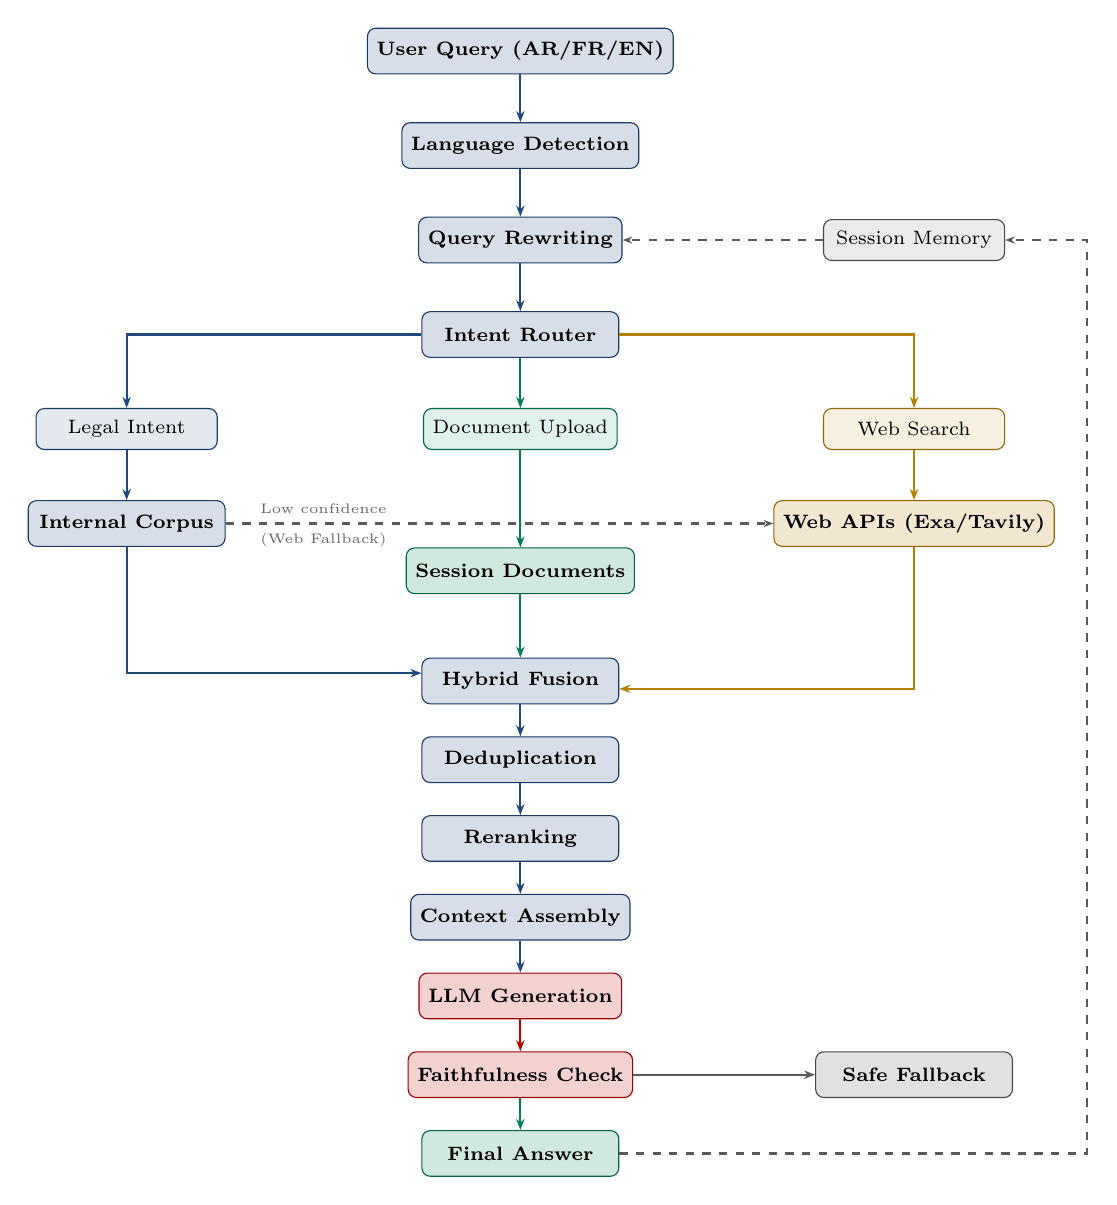
\begin{tikzpicture}[
  x=1cm, y=1cm,
  pipenode/.style 2 args={
    rectangle, rounded corners=3pt,
    minimum width=2.5cm, minimum height=0.58cm,
    text centered, font=\scriptsize\bfseries,
    draw=#1!80!black, fill=#1!18, text=black},
  snode/.style 2 args={
    rectangle, rounded corners=3pt,
    minimum width=2.3cm, minimum height=0.52cm,
    text centered, font=\scriptsize,
    draw=#1!80!black, fill=#1!12, text=black},
  arr/.style={-{Stealth[length=4pt]}, thick, color=#1},
  darr/.style={-{Stealth[length=3.5pt]}, dashed, thick, color=#1}
]

% ── Preprocessing (Center Spine) ──────────────────────────
\node[pipenode={tikzblue}{}] (query)   at (7, 10.0) {\scriptsize User Query (AR/FR/EN)};
\node[pipenode={tikzblue}{}] (lang)    at (7, 8.8)  {\scriptsize Language Detection};
\node[pipenode={tikzblue}{}] (rewrite) at (7, 7.6)  {\scriptsize Query Rewriting};
\node[pipenode={tikzblue}{}] (router)  at (7, 6.4)  {\scriptsize Intent Router};

% ── Memory ────────────────────────────────────────────────
\node[snode={tikzgray}{}] (mem) at (12, 7.6) {\scriptsize Session Memory};

% ── Intent Branches ───────────────────────────────────────
\node[snode={tikzblue}{}]  (legal) at (2, 5.2) {\scriptsize Legal Intent};
\node[snode={tikzgreen}{}] (docs)  at (7, 5.2) {\scriptsize Document Upload};
\node[snode={tikzgold}{}]  (web)   at (12, 5.2) {\scriptsize Web Search};

% ── Sources ───────────────────────────────────────────────
\node[pipenode={tikzblue}{}]  (corpus)    at (2, 4.0) {\scriptsize Internal Corpus};
\node[pipenode={tikzgreen}{}] (user_docs) at (7, 3.4) {\scriptsize Session Documents};
\node[pipenode={tikzgold}{}]  (web_src)   at (12, 4.0) {\scriptsize Web APIs (Exa/Tavily)};

% ── Fusion Pipeline (Center Spine) ────────────────────────
\node[pipenode={tikzblue}{}] (fusion)  at (7, 2.0) {\scriptsize Hybrid Fusion};
\node[pipenode={tikzblue}{}] (dedup)   at (7, 1.0) {\scriptsize Deduplication};
\node[pipenode={tikzblue}{}] (rerank)  at (7, 0.0) {\scriptsize Reranking};
\node[pipenode={tikzblue}{}] (ctx)     at (7, -1.0) {\scriptsize Context Assembly};

% ── Generation & Verification ─────────────────────────────
\node[pipenode={tikzred}{}]   (gen)    at (7, -2.0) {\scriptsize LLM Generation};
\node[pipenode={tikzred}{}]   (faith)  at (7, -3.0) {\scriptsize Faithfulness Check};
\node[pipenode={tikzgreen}{}] (answer) at (7, -4.0) {\scriptsize Final Answer};
\node[pipenode={tikzgray}{}]  (fall)   at (12, -3.0) {\scriptsize Safe Fallback};

% ── Arrows: Spine 1: Preprocessing ────────────────────────────────
\draw[arr={tikzblue}] (query)   -- (lang);
\draw[arr={tikzblue}] (lang)    -- (rewrite);
\draw[arr={tikzblue}] (rewrite) -- (router);

% ── Arrows: Routing Branching ─────────────────────────────────────
\draw[arr={tikzblue}]  (router.west) -| (legal.north);
\draw[arr={tikzgreen}] (router.south) -- (docs.north);
\draw[arr={tikzgold}]  (router.east) -| (web.north);

% ── Arrows: Intents to Sources ────────────────────────────────────
\draw[arr={tikzblue}]  (legal) -- (corpus);
\draw[arr={tikzgreen}] (docs)  -- (user_docs);
\draw[arr={tikzgold}]  (web)   -- (web_src);

% ── Arrows: Web Fallback ──────────────────────────────────────────
\draw[darr={tikzgray}] (corpus.east) -- (web_src.west);
\node[above, font=\tiny, text=black!60] at (4.5, 4.0) {Low confidence};
\node[below, font=\tiny, text=black!60] at (4.5, 4.0) {(Web Fallback)};

% ── Arrows: Sources to Fusion ─────────────────────────────────────
\draw[arr={tikzblue}]  (corpus.south) |- ([yshift= 0.1cm]fusion.west);
\draw[arr={tikzgreen}] (user_docs.south) -- (fusion.north);
\draw[arr={tikzgold}]  (web_src.south) |- ([yshift=-0.1cm]fusion.east);

% ── Arrows: Fusion Pipeline ───────────────────────────────────────
\draw[arr={tikzblue}] (fusion) -- (dedup);
\draw[arr={tikzblue}] (dedup)  -- (rerank);
\draw[arr={tikzblue}] (rerank) -- (ctx);
\draw[arr={tikzblue}] (ctx)    -- (gen);
\draw[arr={tikzred}]  (gen)    -- (faith);

% ── Arrows: Final Branching ───────────────────────────────────────
\draw[arr={tikzgreen}] (faith) -- (answer);
\draw[arr={tikzgray}]  (faith.east) -- (fall.west);

% ── Arrows: Memory Feedback ───────────────────────────────────────
\draw[darr={tikzgray}] (answer.east) -- (14.2, -4.0) |- (mem.east);
\draw[darr={tikzgray}] (mem.west) -- (rewrite.east);

\end{tikzpicture}
\caption{End-to-end RAG pipeline. Solid arrows = main flow; dashed = session memory feedback.}
\label{fig:architecture}
\end{figure}

\subsection{Pipeline Pseudocode}
\label{sec:pseudocode}

The following algorithms formalise the four key stages of the pipeline shown
in Figure~\ref{fig:architecture}.

\begin{lstlisting}[caption={Stage 1 --- Language detection and query preparation.},
                   label={lst:prep}, language={}]
Algorithm PrepareQuery(q_t, history)
  Input : raw query q_t, conversation history H
  Output: standalone query q*, language label lang

  // Stage 1 - Unicode heuristic (fast path)
  arabic_ratio <- count_arabic_chars(q_t) / count_alpha(q_t)
  if arabic_ratio >= 0.30 then
      lang <- "ar"
  else
      // Stage 2 - LLM zero-shot fallback
      lang <- llm_zero_shot_detect(q_t)   // returns "ar"|"fr"|"en"

  // Resolve implicit references using history
  if query_depends_on_history(q_t, H) then
      q* <- llm_rewrite(q_t, H)
  else
      q* <- q_t

  return (q*, lang)
\end{lstlisting}

\begin{lstlisting}[caption={Stage 2 --- Intent classification and routing.},
                   label={lst:intent}, language={}]
Algorithm ClassifyAndRoute(q*, lang)
  Input : standalone query q*, language lang
  Output: routing policy P

  // LLM zero-shot classification
  (intent, confidence) <- llm_classify(q*, lang)
    // intent in {legal_query, document_query, general_knowledge}

  if confidence < THRESHOLD then
      intent <- llm_resolve_ambiguity(q*, lang, intent)

  // Map intent to retrieval channels
  P.internal <- (intent == legal_query)
  P.user_docs <- (intent == document_query)
  P.web       <- (intent == general_knowledge) OR P.internal == False
  P.direct_gen <- (intent == general_knowledge) AND NOT P.web

  return P
\end{lstlisting}

\begin{lstlisting}[caption={Stage 3 --- Multi-source retrieval, fusion, and reranking.},
                   label={lst:retrieval}, language={}]
Algorithm RetrieveAndFuse(q*, lang, P)
  Input : standalone query q*, language lang, policy P
  Output: top-k evidence set E

  D <- {}

  if P.internal then
      D_int  <- dense_search(q*, collection="legal_docs", lang)
                union bm25_search(q*, collection="legal_docs")
      D      <- D union D_int

  if P.user_docs then
      D_usr  <- dense_search(q*, collection="doc_chunks",
                             filter={session, owner})
      D      <- D union D_usr

  if P.web then
      D_web  <- web_search(q*, provider=Exa|Tavily)
      D      <- D union D_web

  // Reciprocal Rank Fusion
  for each d in D:
      d.score <- 1/(60 + rank_dense(d)) + 1/(60 + rank_sparse(d))

  D <- sort_desc(D, key=score)

  // Jaccard deduplication (threshold 0.85)
  D <- deduplicate(D)

  // Cosine reranking
  for each d in D:
      d.score <- cosine(embed(q*), embed(d)) / (norm*norm + 1e-9)

  return top_k(D, k=5)
\end{lstlisting}

\begin{lstlisting}[caption={Stage 4 --- Verified answer generation.},
                   label={lst:gen}, language={}]
Algorithm GenerateVerifiedAnswer(q*, H, E)
  Input : standalone query q*, history H, evidence E
  Output: final answer or safe fallback

  context <- build_context(E, H)   // token-budget truncation applied
  draft   <- llm_generate(q*, context, respond_in=lang)

  verdict <- llm_faithfulness_check(draft, E)
    // returns "faithful" or "not_faithful"

  if verdict == "faithful" then
      persist_session(q*, draft, E)
      return draft
  else
      return SAFE_FALLBACK_MSG
\end{lstlisting}

% ══════════════════════════════════════════════════════════════════════════════
\section{Methodology}
% ══════════════════════════════════════════════════════════════════════════════

\subsection{Language Detection}

The system supports three languages: Arabic, French, and English.
Detection follows a two-stage strategy combining Unicode heuristics with
a zero-shot LLM classifier.

\textbf{Stage 1 --- Unicode Script Analysis.}
Arabic script is detected by computing the ratio of Arabic Unicode characters
(ranges \texttt{U+0600--U+06FF}, \texttt{U+0750--U+077F}, \texttt{U+08A0--U+08FF},
\texttt{U+FB50--U+FDFF}, \texttt{U+FE70--U+FEFF}) to the total number of
alphabetic characters. If this ratio exceeds $0.30$, the query is classified
as Arabic. The threshold of $0.30$ accounts for the frequent presence of French
or English loanwords in modern Arabic text, consistent with thresholds used by
established libraries such as \texttt{langdetect} and \texttt{pycld2}
(typically $0.25$--$0.40$).

\textbf{Stage 2 --- LLM Zero-Shot Detection.}
For non-Arabic text, and as a validation layer for ambiguous inputs, a zero-shot
LLM call is used. The model is prompted to output a single language label
(\texttt{ar}, \texttt{fr}, or \texttt{en}) given the query text. This approach
handles code-mixed inputs (e.g., French queries containing Arabic proper nouns)
more robustly than statistical trigram detectors alone, and eliminates the need
for a separately maintained language model.

\begin{notebox}
Delegating the final language decision to the LLM allows the system to leverage
the same multilingual competence that drives intent classification, creating a
unified zero-shot reasoning layer at the top of the pipeline.
\end{notebox}

\subsection{Contextual Query Rewriting}

In multi-turn conversations, follow-up queries often contain implicit references
(e.g., \textit{``What about the deadlines?''} following a discussion about doctoral
enrollment). Before classification and retrieval, the system rewrites such queries
by incorporating relevant context from the conversation history, producing a
self-contained query suitable for single-turn retrieval.

\subsection{Intent Classification}

The system classifies each query into one of three intent categories:

\begin{itemize}[leftmargin=1.8em, itemsep=0.25em]
  \item \texttt{legal\_query} --- questions about laws, regulations, or administrative
        procedures.
  \item \texttt{document\_query} --- questions about user-uploaded documents.
  \item \texttt{general\_knowledge} --- questions that do not require document retrieval.
\end{itemize}

Classification is performed via a zero-shot LLM call with a structured prompt
that instructs the model to output exactly one intent label. This approach
replaces a previous regex-based heuristic system that suffered from three
limitations: (1) regex patterns were written primarily in English and French,
causing Arabic queries to be misclassified by default; (2) the scoring formula
relied on empirically unvalidated constants; and (3) adding support for new
phrasings required manual pattern engineering.

When the classification confidence is low or the query is ambiguous, a secondary
LLM call triggers an ambiguity resolution step before routing proceeds.

The LLM-based approach natively handles all three languages, requires no
handcrafted rules, and introduces no arbitrary numerical parameters.

\begin{notebox}
By delegating classification to the LLM, the system inherits the model's
multilingual competence. This eliminates the need for language-specific
pattern maintenance and removes all manually tuned scoring constants from
the classification pipeline.
\end{notebox}

\subsection{Query Routing}

Based on the classified intent, the query is routed to the appropriate data source:

\begin{itemize}[leftmargin=1.8em, itemsep=0.2em]
  \item \texttt{legal\_query} $\rightarrow$ vector database,
        \textit{legal\_documents} collection.
  \item \texttt{document\_query} $\rightarrow$ vector database,
        \textit{document\_chunks} collection (session-scoped).
  \item \texttt{general\_knowledge} $\rightarrow$ direct LLM generation
        without retrieval, with optional web fallback.
\end{itemize}

For queries where internal corpora are insufficient, the routing policy may
additionally enable the controlled web search channel described in
Section~\ref{sec:websearch}.

\subsection{Vector Representation}

Document chunks and queries are encoded using BGE-M3~\cite{chen2024bgem3},
a 2024 multilingual embedding model that produces both dense and sparse vector
representations simultaneously. The dense embedding dimension is 1024.

\begin{table}[H]
  \centering
  \caption{Comparison of embedding models.}
  \label{tab:models}
  \begin{tabularx}{\linewidth}{L{3cm} L{4.5cm} Y}
    \rowcolor{tablehead}
    \color{white}\textbf{Aspect} &
    \color{white}\textbf{Previous Model} &
    \color{white}\textbf{Current Model} \\
    \rowcolor{lightblue}
    Name         & \texttt{mpnet-base-v2}            & \texttt{BAAI/BGE-M3} \\
    Year         & 2019                              & 2024 \\
    \rowcolor{lightblue}
    Outputs      & Dense 768d only                   & Dense 1024d + Sparse \\
    Arabic support & Limited                         & Advanced (extended corpus) \\
    \rowcolor{lightblue}
    Reference    & Reimers \& Gurevych~\cite{reimers2019sbert} &
                   Chen et al.~\cite{chen2024bgem3} \\
  \end{tabularx}
\end{table}

\subsection{Hybrid Retrieval with Reciprocal Rank Fusion}

A purely semantic retrieval approach fails on queries containing exact statutory
references.

\begin{failurebox}
For a query such as \textit{``Article 43 of Executive Decree 05-315''}, dense embeddings
encode ``Article~43'' and ``Article~44'' in quasi-identical vector regions. Semantic
search alone cannot distinguish these exact references. BM25 resolves this trivially
via exact token matching.
\end{failurebox}

The system therefore employs a true hybrid retrieval strategy with two components:

\textbf{Dense retrieval} uses the BGE-M3 dense embeddings to capture semantic
similarity via cosine distance over the Qdrant vector index.

\textbf{Sparse retrieval} uses BM25 scoring with standard parameters
$(k_1 = 1.5,\ b = 0.75)$ as established by Robertson and Zaragoza~\cite{robertson2009bm25}.

The two ranked lists are merged using Reciprocal Rank Fusion~\cite{cormack2009rrf}:

\begin{equation}
  \mathrm{RRF}(d) = \frac{1}{k + \mathrm{rank}_{\mathrm{dense}}(d)}
                  + \frac{1}{k + \mathrm{rank}_{\mathrm{sparse}}(d)}
  \label{eq:rrf}
\end{equation}

where $k = 60$ is the standard constant from the original RRF paper. This fusion
method requires no tuning of interpolation weights and has been shown to outperform
individual ranking methods as well as learned fusion approaches~\cite{cormack2009rrf}.

\subsection{Deduplication}

Hybrid retrieval may return near-duplicate passages retrieved by both the dense
and sparse components. Duplicates are identified using the Jaccard similarity
coefficient over token sets:

\begin{equation}
  J(A, B) = \frac{|A \cap B|}{|A \cup B|}
  \label{eq:jaccard}
\end{equation}

Pairs with $J(A,B) \geq 0.85$ are considered duplicates, and the lower-scoring
passage is removed. The threshold of $0.85$ follows established practice in
web-scale deduplication~\cite{manku2007neardup}.

\subsection{Reranking and Context Construction}

The deduplicated candidate set is reranked by cosine similarity between the query
embedding and each passage embedding:

\begin{equation}
  \mathrm{score}(q, d) = \frac{\mathbf{q} \cdot \mathbf{d}}
                              {\|\mathbf{q}\| \cdot \|\mathbf{d}\| + \varepsilon}
  \label{eq:cosine}
\end{equation}

where $\varepsilon = 10^{-9}$ ensures numerical stability. The \textbf{top-5
passages} are selected for context construction.

To ensure coverage across multiple source documents, a balanced selection policy
guarantees a minimum of 2 chunks per source document before filling remaining
slots by score.

\subsection{LLM Generation}

The selected passages, the rewritten query, and a summary of the conversation
history are assembled into a structured prompt. The LLM is instructed to:
(1) generate a response grounded in the provided context,
(2) cite specific legal articles where applicable, and
(3) respond in the same language as the user's query.

\subsection{Faithfulness Verification}

As a final safeguard, the generated response is verified against the retrieved
context through a secondary LLM call. The verification prompt presents both the
context and the generated response, and asks whether every factual claim in the
response is supported by the context. The model outputs a binary judgment:
\texttt{faithful} or \texttt{not\_faithful}.

If the response is judged unfaithful, the system returns a fallback message
indicating that a reliable answer could not be found in the available legal
documents.

\begin{warningbox}
A legal chatbot that presents hallucinated information with confidence is more
dangerous than one that acknowledges uncertainty. The faithfulness check
constitutes the \textbf{last line of defense} against legal hallucinations.
\end{warningbox}

% ══════════════════════════════════════════════════════════════════════════════
\section{Controlled Web Search}
\label{sec:websearch}
% ══════════════════════════════════════════════════════════════════════════════

Web retrieval is treated as a \textit{controlled expansion} channel, not as a
default behavior. It is useful when the internal legal corpus does not contain
recent amendments, newly published decrees, or domain-specific content that has
not yet been indexed. The system integrates two independent web search providers
--- Exa and Tavily --- each exposed through a distinct integration mode.

\subsection{Web Search Providers}

\subsubsection{Exa --- Semantic Neural Search}

Exa (\texttt{exa.ai}) is a neural search engine designed for LLM-augmented
pipelines. Unlike keyword-based engines, Exa encodes queries using embeddings
and retrieves semantically matching web pages, making it well-suited for legal
paraphrase matching and conceptual queries.

Key theoretical characteristics in this architecture:
\begin{itemize}[leftmargin=1.8em, itemsep=0.2em]
  \item \textbf{Query type:} neural (embedding-based retrieval over web content).
  \item \textbf{Output format:} ranked list of URLs with semantically extracted source highlights.
  \item \textbf{Integration mode:} acts as an automatic pipeline fallback when internal
        corpus evidence is theoretically evaluated as insufficient by the routing policy.
  \item \textbf{Strengths:} handles paraphrastic legal queries and retrieves
        full-text content from authoritative online legal sources.
\end{itemize}

Exa results are chunked, embedded with BGE-M3, and enter the RRF fusion
pipeline as a scored candidate set alongside internal corpus passages.
They are \emph{not} appended to the context unconditionally.

\subsubsection{Tavily --- User-Triggered Search Button}

Tavily (\texttt{tavily.com}) is a search API built specifically for AI agents.
It returns pre-extracted, AI-ready snippets optimised for direct injection into
LLM prompts, with built-in source filtering to favour authoritative domains.

In this conceptual model, Tavily represents the \textbf{user-triggered web search
channel}. When a user explicitly shifts intent toward external web knowledge,
the standard internal RAG flow is bypassed, and Tavily serves as the direct pipeline:

\begin{itemize}[leftmargin=1.8em, itemsep=0.2em]
  \item \textbf{Trigger:} explicit user delegation to external search via the interaction interface.
  \item \textbf{Behaviour:} bypasses the internal indexed corpus to retrieve live web
        evidence reflecting current events or extremely recent modifications to the law.
  \item \textbf{Output format:} AI-ready text snippets with authoritative source URLs.
  \item \textbf{Strengths:} minimized latency and provision of pre-filtered snippets, ensuring
        rapid response for real-time legal queries.
\end{itemize}

\begin{webbox}
\textbf{Exa} is activated \emph{automatically} by the routing policy when
internal evidence is weak. \textbf{Tavily} is activated \emph{explicitly}
by the user pressing the web search button. Both channels pass through the
same faithfulness verification gate before a response is returned.
\end{webbox}

\subsection{Integration Modes}

\textbf{Mode 1 --- Automatic pipeline fallback (Exa).}
When routing policy determines that internal retrieval evidence is insufficient
for a given query, the system activates Exa. Results are fetched, chunked, and
passed through the same deduplication and reranking stages as internal passages
before context assembly.

\textbf{Mode 2 --- User-triggered web search (Tavily).}
The user explicitly orchestrates a web-grounded query via the conversational interface.
The pipeline directly constructs a web-grounded answer using Tavily's real-time
retrieval, bypassing the internal corpus entirely to guarantee the inclusion of
the most contemporaneous external perspectives.

\subsection{Shared Policy Constraints}

Key constraints that apply to both providers:

\begin{enumerate}[leftmargin=1.8em, itemsep=0.2em]
  \item Web retrieval is activated only when routing policy or explicit user
        action permits it.
  \item Web evidence is scored and ranked through the same RRF pipeline as
        internal corpus evidence; it is never appended unconditionally.
  \item The faithfulness verification module applies to web-grounded answers
        with the same binary \texttt{faithful}/\texttt{not\_faithful} standard.
  \item The system does not expose raw web content to the user; all answers
        are generated by the LLM and verified before delivery.
\end{enumerate}

\begin{table}[H]
  \centering
  \caption{Comparison of web search providers.}
  \label{tab:webproviders}
  \begin{tabularx}{\linewidth}{L{2.5cm} L{4.5cm} Y}
    \rowcolor{tablehead}
    \color{white}\textbf{Aspect} &
    \color{white}\textbf{Exa} &
    \color{white}\textbf{Tavily} \\
    \rowcolor{lightblue}
    Search type    & Neural (embedding-based)      & Keyword + AI-filtered \\
    Trigger        & Automatic (policy fallback)   & User button in UI \\
    \rowcolor{lightblue}
    Output format  & URL + extracted highlights    & Pre-extracted snippets \\
    Streaming      & No                            & Yes (SSE) \\
    \rowcolor{lightblue}
    Best for       & Semantic / paraphrase queries & Current events, fast lookup \\
    Role in Pipeline & Fallback augmentation         & Primary external stream \\
  \end{tabularx}
\end{table}

% ══════════════════════════════════════════════════════════════════════════════
\section{User Document Ingestion}
% ══════════════════════════════════════════════════════════════════════════════

User document uploading enables personalized, session-scoped grounding. In many
legal-administrative scenarios, the most relevant evidence is not in global corpora
but in local files such as institutional circulars, administrative forms, or
internal regulations.

The ingestion pipeline is executed asynchronously to preserve interactive response
latency. It consists of four sequential steps:

\begin{enumerate}[leftmargin=1.8em, itemsep=0.2em]
  \item \textbf{Extraction} --- text is extracted from uploaded files
        (PDF, DOCX, XLSX, or plain text) using format-specific processors.
  \item \textbf{Chunking} --- extracted text is segmented using the same
        structure-aware strategy described in Section~\ref{sec:chunking}.
  \item \textbf{Embedding} --- each chunk is encoded with BGE-M3 to produce
        dense and sparse vectors.
  \item \textbf{Indexing} --- chunks and vectors are persisted in the vector
        database under the user's session and ownership scope, ensuring strict
        isolation from other users' documents.
\end{enumerate}

Once ingested, user documents are retrieved through the standard hybrid pipeline
with session-scoped filters applied. A balanced selection policy ensures coverage
across multiple uploaded files within the same session.

% ══════════════════════════════════════════════════════════════════════════════
\section{Document Processing}
\label{sec:chunking}
% ══════════════════════════════════════════════════════════════════════════════

\subsection{Structure-Aware Chunking}

Legal documents have a well-defined hierarchical structure (parts, chapters,
articles, paragraphs). A fixed-size chunking strategy risks splitting an article
across two chunks, destroying its semantic coherence. The system employs a
hierarchical chunking strategy that respects document structure:

\begin{table}[H]
  \centering
  \caption{Hierarchical chunking priority levels.}
  \label{tab:chunking}
  \begin{tabularx}{\linewidth}{C{1.2cm} L{3.5cm} Y}
    \rowcolor{tablehead}
    \color{white}\textbf{Priority} &
    \color{white}\textbf{Boundary Type} &
    \color{white}\textbf{Detection Patterns} \\
    \rowcolor{lightblue}
    1 & Legal article boundaries &
        Article X, Art. X (French); Arabic article markers \\
    2 & Paragraph boundaries & Double line breaks \\
    \rowcolor{lightblue}
    3 & Sentence boundaries & Terminal punctuation (. ?) \\
    4 & Token-level fallback & 512 tokens with 64-token overlap (12.5\%) \\
  \end{tabularx}
\end{table}

The fallback chunk size of 512 tokens corresponds to the input limit of
BERT-family models. The 12.5\% overlap ensures contextual continuity between
adjacent chunks, following the practice established in the original RAG
work~\cite{lewis2020rag}.

\subsection{Chunking Parameters}

\begin{table}[H]
  \centering
  \caption{Document chunking and retrieval parameters.}
  \label{tab:params}
  \begin{tabularx}{\linewidth}{L{3.5cm} L{3.5cm} Y}
    \rowcolor{tablehead}
    \color{white}\textbf{Parameter} &
    \color{white}\textbf{Value} &
    \color{white}\textbf{Justification} \\
    \rowcolor{lightblue}
    Strategy       & Structure-aware       & Preserves legal article boundaries \\
    Chunk size     & 512 tokens            & BERT-family model input limit \\
    \rowcolor{lightblue}
    Chunk overlap  & 64 tokens (12.5\%)   & Contextual continuity~\cite{lewis2020rag} \\
    Top-$K$        & 5                     & LLM context budget, standard RAG practice \\
    \rowcolor{lightblue}
    Min.\ per document & 2 chunks          & Multi-document coverage guarantee \\
  \end{tabularx}
\end{table}

% ══════════════════════════════════════════════════════════════════════════════
\section{Evaluation}
% ══════════════════════════════════════════════════════════════════════════════

The system is evaluated along two axes: retrieval quality and generation quality.
Three evaluation scenarios are used to isolate the contribution of individual
pipeline components: a \textit{baseline} retrieval scenario, a
\textit{reranker\_top5} scenario, and an \textit{exa\_fallback\_top5} scenario
activating the web search fallback.

\subsection{Retrieval Metrics}

Three standard information retrieval metrics are used:

\textbf{Precision@$k$} measures the fraction of retrieved documents in the
top-$k$ results that are relevant:
\begin{equation}
  \text{Precision@}k = \frac{|\{\text{relevant documents}\} \cap \{\text{top-}k \text{ retrieved documents}\}|}{k}
\end{equation}

\textbf{Recall@$k$} measures the fraction of all relevant documents that appear
in the top-$k$ results:
\begin{equation}
  \text{Recall@}k = \frac{|\{\text{relevant documents}\} \cap \{\text{top-}k \text{ retrieved documents}\}|}{|\{\text{relevant documents}\}|}
\end{equation}

\textbf{Mean Reciprocal Rank (MRR)} captures how quickly the first relevant
document appears in the ranked list, computed as the average of the reciprocal
of the rank of the first relevant result across all queries:
\begin{equation}
  \mathrm{MRR} = \frac{1}{|Q|} \sum_{i=1}^{|Q|} \frac{1}{\mathrm{rank}_i}
\end{equation}
where $Q$ is the set of queries and $\mathrm{rank}_i$ is the rank position of the first relevant document for the $i$-th query.

\subsection{Generation Metrics}

BERTScore~\cite{zhang2020bertscore} is used as the primary automated generation
metric. It computes token-level cosine similarities between contextual embeddings
of the generated and reference texts, providing a semantic similarity measure
that is more robust across languages than lexical overlap metrics such as BLEU
or ROUGE.

\subsection{Human Evaluation}

Automated metrics are complemented by human evaluation along five dimensions:

\begin{table}[H]
  \centering
  \caption{Human evaluation criteria.}
  \label{tab:human}
  \begin{tabularx}{\linewidth}{L{3.5cm} Y}
    \rowcolor{tablehead}
    \color{white}\textbf{Criterion} &
    \color{white}\textbf{Description} \\
    \rowcolor{lightblue}
    Legal correctness &
        Whether the legal information provided is accurate \\
    Completeness &
        Whether all relevant aspects of the question are covered \\
    \rowcolor{lightblue}
    Clarity &
        Whether the response is understandable by a non-expert \\
    Source citation &
        Whether references to specific legal texts are provided \\
    \rowcolor{lightblue}
    Safe fallback &
        Whether the system appropriately declines when evidence
        is insufficient \\
  \end{tabularx}
\end{table}

% ══════════════════════════════════════════════════════════════════════════════
\section{Discussion}
% ══════════════════════════════════════════════════════════════════════════════

The architectural decisions described in this paper address several specific
challenges in multilingual legal information retrieval.

\textbf{Hybrid retrieval} resolves the fundamental tension between semantic
understanding and exact reference matching. Legal queries frequently contain
precise statutory identifiers (e.g., ``Article 43 of Executive Decree 05-315'')
that dense embeddings cannot reliably distinguish. The combination of dense and
sparse retrieval via RRF ensures that both query types are handled effectively
without introducing tunable interpolation weights.

\textbf{LLM-based language detection and intent classification} eliminate the
maintenance burden and language coverage gaps inherent in rule-based approaches.
The previous regex-based system required manual pattern engineering for each
language and relied on scoring constants that had not been validated on real
user data. The zero-shot LLM approach handles all three languages natively and
introduces no arbitrary parameters.

\textbf{Structure-aware chunking} preserves the semantic integrity of legal
articles, which are the fundamental units of legal reasoning. Splitting an
article across chunks risks losing critical context, such as conditions or
exceptions stated later in the same article.

\textbf{Controlled web search} extends the system's effective knowledge
boundary without compromising answer reliability. By treating web evidence
as a scored candidate channel subject to the same faithfulness gate as
internal corpus evidence, the system avoids the uncontrolled noise
propagation that would result from naive web augmentation.

\textbf{Faithfulness verification} provides a critical safety mechanism for
a legal application. A system that presents hallucinated legal information
with confidence is more harmful than one that acknowledges uncertainty.
The binary faithful/unfaithful check with a safe fallback ensures that users
are not misled.

\subsection{Limitations}

The system relies on the quality and completeness of the indexed legal corpus:
documents not included in the index cannot be retrieved without activating
web fallback. The faithfulness verification module adds latency through an
additional LLM call. Furthermore, the current evaluation framework has not
yet been applied to a large-scale user study, which would be necessary to
validate the system's effectiveness in practice. Web retrieval introduces
additional latency and dependency on external service availability.

% ══════════════════════════════════════════════════════════════════════════════
\section{Conclusion}
% ══════════════════════════════════════════════════════════════════════════════

This paper presented the architecture of a multilingual legal chatbot based on
Retrieval-Augmented Generation. The system processes queries in Arabic, French,
and English through a ten-stage pipeline that includes LLM-based zero-shot
language detection, contextual query rewriting, LLM-based intent classification,
hybrid dense--sparse retrieval with Reciprocal Rank Fusion, controlled web-search
augmentation, user document ingestion, structure-aware document chunking, and
post-generation faithfulness verification.

The design prioritizes factual grounding and safe failure modes, which are
essential properties for any system operating in the legal domain. Future work
includes conducting a comprehensive user study, exploring cross-lingual retrieval
where the query language differs from the document language, investigating
fine-tuned reranking models to further improve retrieval precision, and
evaluating more sophisticated faithfulness verification approaches beyond
binary classification.

% ══════════════════════════════════════════════════════════════════════════════
\newpage
\begin{thebibliography}{99}

\bibitem{lewis2020rag}
P. Lewis, E. Perez, A. Piktus, F. Petroni, V. Karpukhin, N. Goyal, H. K{\"u}ttler,
M. Lewis, W.-t. Yih, T. Rockt{\"a}schel, S. Riedel, and D. Kiela,
``Retrieval-Augmented Generation for Knowledge-Intensive NLP Tasks,''
\textit{Advances in Neural Information Processing Systems (NeurIPS)}, 2020.

\bibitem{robertson2009bm25}
S. Robertson and H. Zaragoza,
``The Probabilistic Relevance Framework: BM25 and Beyond,''
\textit{Foundations and Trends in Information Retrieval},
vol.~3, no.~4, pp.~333--389, 2009.

\bibitem{cormack2009rrf}
G.~V. Cormack, C.~L.~A. Clarke, and S. Buettcher,
``Reciprocal Rank Fusion Outperforms Condorcet and Individual Rank Learning Methods,''
\textit{Proc. 32nd International ACM SIGIR Conference}, 2009.

\bibitem{bruch2022fusion}
S. Bruch, A. Gai, and A. Ingber,
``An Analysis of Fusion Functions for Hybrid Retrieval,''
\textit{arXiv preprint arXiv:2210.11934}, 2022.

\bibitem{reimers2019sbert}
N. Reimers and I. Gurevych,
``Sentence-BERT: Sentence Embeddings using Siamese BERT-Networks,''
\textit{Proc. EMNLP}, 2019.

\bibitem{chen2024bgem3}
J. Chen, S. Xiao, P. Zhang, K. Luo, D. Lian, and Z. Liu,
``BGE M3-Embedding: Multi-Lingual, Multi-Functionality, Multi-Granularity
Text Embeddings Through Self-Knowledge Distillation,''
\textit{arXiv preprint arXiv:2309.07597}, 2024.

\bibitem{zhang2020bertscore}
T. Zhang, V. Kishore, F. Wu, K.~Q. Weinberger, and Y. Artzi,
``BERTScore: Evaluating Text Generation with BERT,''
\textit{International Conference on Learning Representations (ICLR)}, 2020.

\bibitem{manku2007neardup}
G.~S. Manku, A. Jain, and A.~D. Sarma,
``Detecting Near-Duplicates for Web Crawling,''
\textit{Proc. 16th International Conference on World Wide Web (WWW)}, 2007.

\bibitem{nogueira2019rerank}
R. Nogueira and K. Cho,
``Passage Re-ranking with BERT,''
\textit{arXiv preprint arXiv:1901.04085}, 2019.

\bibitem{salton1983ir}
G. Salton and M.~J. McGill,
\textit{Introduction to Modern Information Retrieval},
McGraw-Hill, 1983.

\bibitem{gao2024ragsurvey}
Y. Gao, Y. Xiong, X. Gao, K. Jia, J. Pan, Y. Bi, Y. Dai, J. Sun, M. Wang, and H. Wang,
``Retrieval-Augmented Generation for Large Language Models: A Survey,''
\textit{arXiv preprint arXiv:2312.10997}, 2024.

\bibitem{karpukhin2020dpr}
V. Karpukhin, B. O\u{g}uz, S. Min, P. Lewis, L. Wu, S. Edunov,
D. Chen, and W.-t. Yih,
``Dense Passage Retrieval for Open-Domain Question Answering,''
\textit{Proc. EMNLP}, 2020.

\bibitem{chalkidis2020legalbert}
I. Chalkidis, M. Fergadiotis, P. Malakasiotis, N. Aletras, and I. Androutsopoulos,
``LEGAL-BERT: The Muppets Straight Out of Law School,''
\textit{Findings of EMNLP}, 2020.

\bibitem{zheng2021lawformer}
C. Zheng, J. Guim, and M. Huang,
``Lawformer: A Pre-trained Language Model for Chinese Legal Long Documents,''
\textit{AI Open}, vol.~2, pp.~79--88, 2021.

\bibitem{min2023factscore}
S. Min, K. Krishna, X. Lyu, M. Lewis, W.-t. Yih, P. Koh, M. Iyyer,
L. Zettlemoyer, and H. Hajishirzi,
``FActScore: Fine-Grained Atomic Evaluation of Factual Precision in Long-Form
Text Generation,''
\textit{Proc. EMNLP}, 2023.

\bibitem{lazaridou2022internetaugmented}
A. Lazaridou, E. Gribovskaya, W. Stokowiec, and N. Grigorev,
``Internet-Augmented Language Models Through Few-Shot Prompting for Open-Domain
Question Answering,''
\textit{arXiv preprint arXiv:2203.05115}, 2022.

\end{thebibliography}

\end{document}
